% Options for packages loaded elsewhere
\PassOptionsToPackage{unicode}{hyperref}
\PassOptionsToPackage{hyphens}{url}
\PassOptionsToPackage{dvipsnames,svgnames,x11names}{xcolor}
%
\documentclass[
  letterpaper,
  DIV=11,
  numbers=noendperiod]{scrartcl}

\usepackage{amsmath,amssymb}
\usepackage{iftex}
\ifPDFTeX
  \usepackage[T1]{fontenc}
  \usepackage[utf8]{inputenc}
  \usepackage{textcomp} % provide euro and other symbols
\else % if luatex or xetex
  \usepackage{unicode-math}
  \defaultfontfeatures{Scale=MatchLowercase}
  \defaultfontfeatures[\rmfamily]{Ligatures=TeX,Scale=1}
\fi
\usepackage{lmodern}
\ifPDFTeX\else  
    % xetex/luatex font selection
\fi
% Use upquote if available, for straight quotes in verbatim environments
\IfFileExists{upquote.sty}{\usepackage{upquote}}{}
\IfFileExists{microtype.sty}{% use microtype if available
  \usepackage[]{microtype}
  \UseMicrotypeSet[protrusion]{basicmath} % disable protrusion for tt fonts
}{}
\makeatletter
\@ifundefined{KOMAClassName}{% if non-KOMA class
  \IfFileExists{parskip.sty}{%
    \usepackage{parskip}
  }{% else
    \setlength{\parindent}{0pt}
    \setlength{\parskip}{6pt plus 2pt minus 1pt}}
}{% if KOMA class
  \KOMAoptions{parskip=half}}
\makeatother
\usepackage{xcolor}
\usepackage{soul}
\setlength{\emergencystretch}{3em} % prevent overfull lines
\setcounter{secnumdepth}{-\maxdimen} % remove section numbering
% Make \paragraph and \subparagraph free-standing
\ifx\paragraph\undefined\else
  \let\oldparagraph\paragraph
  \renewcommand{\paragraph}[1]{\oldparagraph{#1}\mbox{}}
\fi
\ifx\subparagraph\undefined\else
  \let\oldsubparagraph\subparagraph
  \renewcommand{\subparagraph}[1]{\oldsubparagraph{#1}\mbox{}}
\fi


\providecommand{\tightlist}{%
  \setlength{\itemsep}{0pt}\setlength{\parskip}{0pt}}\usepackage{longtable,booktabs,array}
\usepackage{calc} % for calculating minipage widths
% Correct order of tables after \paragraph or \subparagraph
\usepackage{etoolbox}
\makeatletter
\patchcmd\longtable{\par}{\if@noskipsec\mbox{}\fi\par}{}{}
\makeatother
% Allow footnotes in longtable head/foot
\IfFileExists{footnotehyper.sty}{\usepackage{footnotehyper}}{\usepackage{footnote}}
\makesavenoteenv{longtable}
\usepackage{graphicx}
\makeatletter
\def\maxwidth{\ifdim\Gin@nat@width>\linewidth\linewidth\else\Gin@nat@width\fi}
\def\maxheight{\ifdim\Gin@nat@height>\textheight\textheight\else\Gin@nat@height\fi}
\makeatother
% Scale images if necessary, so that they will not overflow the page
% margins by default, and it is still possible to overwrite the defaults
% using explicit options in \includegraphics[width, height, ...]{}
\setkeys{Gin}{width=\maxwidth,height=\maxheight,keepaspectratio}
% Set default figure placement to htbp
\makeatletter
\def\fps@figure{htbp}
\makeatother

\KOMAoption{captions}{tableheading}
\makeatletter
\@ifpackageloaded{tcolorbox}{}{\usepackage[skins,breakable]{tcolorbox}}
\@ifpackageloaded{fontawesome5}{}{\usepackage{fontawesome5}}
\definecolor{quarto-callout-color}{HTML}{909090}
\definecolor{quarto-callout-note-color}{HTML}{0758E5}
\definecolor{quarto-callout-important-color}{HTML}{CC1914}
\definecolor{quarto-callout-warning-color}{HTML}{EB9113}
\definecolor{quarto-callout-tip-color}{HTML}{00A047}
\definecolor{quarto-callout-caution-color}{HTML}{FC5300}
\definecolor{quarto-callout-color-frame}{HTML}{acacac}
\definecolor{quarto-callout-note-color-frame}{HTML}{4582ec}
\definecolor{quarto-callout-important-color-frame}{HTML}{d9534f}
\definecolor{quarto-callout-warning-color-frame}{HTML}{f0ad4e}
\definecolor{quarto-callout-tip-color-frame}{HTML}{02b875}
\definecolor{quarto-callout-caution-color-frame}{HTML}{fd7e14}
\makeatother
\makeatletter
\makeatother
\makeatletter
\makeatother
\makeatletter
\@ifpackageloaded{caption}{}{\usepackage{caption}}
\AtBeginDocument{%
\ifdefined\contentsname
  \renewcommand*\contentsname{Table of contents}
\else
  \newcommand\contentsname{Table of contents}
\fi
\ifdefined\listfigurename
  \renewcommand*\listfigurename{List of Figures}
\else
  \newcommand\listfigurename{List of Figures}
\fi
\ifdefined\listtablename
  \renewcommand*\listtablename{List of Tables}
\else
  \newcommand\listtablename{List of Tables}
\fi
\ifdefined\figurename
  \renewcommand*\figurename{Figure}
\else
  \newcommand\figurename{Figure}
\fi
\ifdefined\tablename
  \renewcommand*\tablename{Table}
\else
  \newcommand\tablename{Table}
\fi
}
\@ifpackageloaded{float}{}{\usepackage{float}}
\floatstyle{ruled}
\@ifundefined{c@chapter}{\newfloat{codelisting}{h}{lop}}{\newfloat{codelisting}{h}{lop}[chapter]}
\floatname{codelisting}{Listing}
\newcommand*\listoflistings{\listof{codelisting}{List of Listings}}
\makeatother
\makeatletter
\@ifpackageloaded{caption}{}{\usepackage{caption}}
\@ifpackageloaded{subcaption}{}{\usepackage{subcaption}}
\makeatother
\makeatletter
\@ifpackageloaded{tcolorbox}{}{\usepackage[skins,breakable]{tcolorbox}}
\makeatother
\makeatletter
\@ifundefined{shadecolor}{\definecolor{shadecolor}{rgb}{.97, .97, .97}}
\makeatother
\makeatletter
\makeatother
\makeatletter
\makeatother
\ifLuaTeX
  \usepackage{selnolig}  % disable illegal ligatures
\fi
\IfFileExists{bookmark.sty}{\usepackage{bookmark}}{\usepackage{hyperref}}
\IfFileExists{xurl.sty}{\usepackage{xurl}}{} % add URL line breaks if available
\urlstyle{same} % disable monospaced font for URLs
\hypersetup{
  pdftitle={BSTA 513/613 Syllabus},
  colorlinks=true,
  linkcolor={blue},
  filecolor={Maroon},
  citecolor={Blue},
  urlcolor={Blue},
  pdfcreator={LaTeX via pandoc}}

\title{BSTA 513/613 Syllabus}
\author{}
\date{}

\begin{document}
\maketitle
\ifdefined\Shaded\renewenvironment{Shaded}{\begin{tcolorbox}[interior hidden, boxrule=0pt, enhanced, borderline west={3pt}{0pt}{shadecolor}, breakable, frame hidden, sharp corners]}{\end{tcolorbox}}\fi

\hypertarget{description}{%
\subsection{Description}\label{description}}

Welcome to BSTA 513/613! In this course, we will continue to learn about
regression analysis, but not with categorical outcomes. We will build
some theoretical understanding in order to interpret and apply logistic
regression models appropriately. We will learn how to build a logistic
regression model, interpret the model and coefficients, and diagnose
potential issues with our model.

\hypertarget{course-learning-objectives}{%
\subsubsection{Course Learning
Objectives}\label{course-learning-objectives}}

At the end of this course, students should be able to\ldots{}

\begin{enumerate}
\def\labelenumi{\arabic{enumi}.}
\item
  Apply and interpret a variety of hypothesis-testing procedures for
  two-way and three-way contingency tables
\item
  Compute and interpret measures of association for binary and ordinal
  data.
\item
  Calculate and correctly interpret odds ratios using logistic
  regression, make comparison across groups and examine relationship
  between binary outcome and predictor variables.
\item
  Apply appropriate model-building strategies for logistic regression.
  Effectively use statistical computing packages for contingency table
  and logistic regression procedures.
\item
  Perform Poisson regression analysis using count data and interpret
  model estimates, make comparison across groups and examine
  relationship between outcome and predictor variables.
\item
  Coherently summarize methods and results of data analyses, and discuss
  in context of original health-related research questions to audiences
  with varied statistical background.
\end{enumerate}

These learning objectives were adapted from
\href{https://maria-tackett.netlify.app/project/02_sta210/}{Maria
Tackett's Regression Analysis course}.

\hypertarget{instructors}{%
\subsection{Instructors}\label{instructors}}

\href{instructors.qmd}{Here is the instructor page.} This also has
office hours!

\hypertarget{meeting-times}{%
\subsection{Meeting Times}\label{meeting-times}}

Mondays~~~~~~~~~~1:00 PM -- 2:50 PM PST in RLSB 3A003 A/B

Wednesdays~~~~1:00 PM -- 2:50 PM PST in RLSB 3A003 A/B

Here is the full schedule:

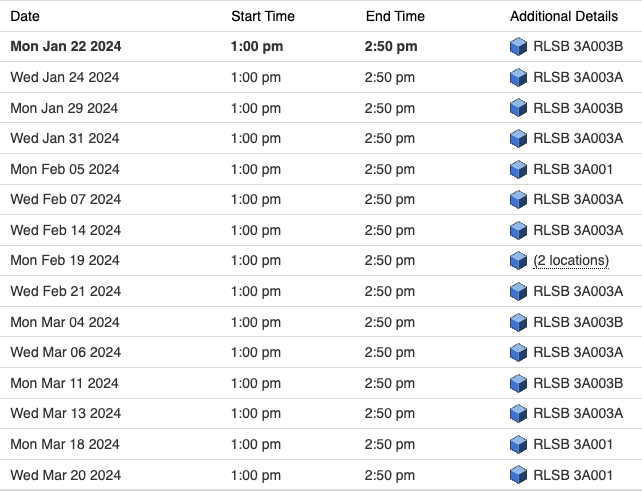
\includegraphics{images/room_sched.png}

\hypertarget{known-exceptions}{%
\subsubsection{Known Exceptions}\label{known-exceptions}}

Monday, February 26~ ~ ~~ ~ ~ ~ ~1:00 PM -- 2:50 PM PST \textbf{on Webex
OR pre-recorded}

Wednesday, February 28~ ~ ~~ ~1:00 PM -- 2:50 PM PST \textbf{on Webex OR
pre-recorded}

\hypertarget{materials}{%
\subsection{Materials}\label{materials}}

\hypertarget{textbooks}{%
\subsubsection{Textbooks}\label{textbooks}}

In lieu of a formally published textbook, we will be referencing the
following two online textbooks. Similar to our class, the books
integrate R into their lessons.

\begin{itemize}
\item
  \href{https://jfrench.github.io/LinearRegression/}{A Progressive
  Introduction to Linear Models} by Joshua French
\item
  \href{https://bookdown.org/rwnahhas/RMPH/}{Introduction to Regression
  Methods for Public Health Using R} by Ramzi W. Nahhas
\end{itemize}

\hypertarget{supplemental-readings-optional}{%
\paragraph{Supplemental Readings
(Optional)}\label{supplemental-readings-optional}}

\begin{itemize}
\tightlist
\item
  \emph{An Introduction to R}
  (\href{http://cran.r-project.org/manuals.html}{free pdf available})
\end{itemize}

\hypertarget{online-resources}{%
\subsubsection{Online Resources}\label{online-resources}}

\hypertarget{slack}{%
\paragraph{Slack}\label{slack}}

We will use Slack as our main form of communication for the class. If
you are unsure how to do a homework problem or have other questions,
please ask me by posting your question(s) on Slack. Please know that
Slack is not guarded by the OSHU firewall, so if you have a question
about accommodations or any sensitive topics, you may wish to message me
via email. You can still message me regarding sensitive information on
Slack, but I will not initiate those conversations on Slack.

\href{https://join.slack.com/t/slack-xvk6383/shared_invite/zt-29g7biioz-XhPs~tj8xwL1GajEw9YlTg}{**Please
use this invitation link for our Slack workspace!**}

\textbf{Tips on asking questions:}

\begin{itemize}
\tightlist
\item
  When reaching out for help for a homework problem, please include some
  context on what you have already tried.

  \begin{itemize}
  \tightlist
  \item
    For example, including a photo of your work thus far with an
    explanation of where you think you might be wrong is a quick way for
    me to look over your work and help you troubleshoot. This helps me
    see what parts you already understand and which you need help with.
    If your question involves code, please \textbf{include the copied
    code (not a screenshot)} and an attachment to your full file. This
    way I can see the exact line you need help with and the full code in
    case the problem starts earlier.
  \item
    If you are unsure how to start a problem, look through your notes
    and the book for examples that you think might be similar. When
    reaching out, mention these examples and why you think they might be
    helpful, but also why you are still unsure on how to proceed.
  \item
    If you only write something similar to ``I don't know how to do
    problem xxx,'' then my response will be to ask you what you tried so
    far. Thus, it will be quicker for you to let me know this
    information right away.
  \end{itemize}
\item
  If asking for help about a specific example that you don't understand,
  please also provide some detail beyond ``I don't understand example
  xxx.''

  \begin{itemize}
  \tightlist
  \item
    Which steps of the problem do you not understand? You can refer to a
    line number, for example.
  \item
    If you don't understand the first step, do you understand the ones
    following it?
  \end{itemize}
\item
  In general, when asking a question, please provide the homework number
  it is from along with the chapter and problem number. If it's an
  example from the notes or book, an example number or slide number will
  help finding it.
\item
  Want more tips on asking questions? This list on
  \href{https://www.weareteachers.com/8-ways-to-pose-better-questions-in-math-class/}{this
  site} will help!
\item
  Finally, if I don't respond within a day and you need a response soon,
  \emph{please remind me by emailing or messaging me again}.
\end{itemize}

\hypertarget{sakai}{%
\paragraph{Sakai}\label{sakai}}

While most course materials will be delivered online through this
website, assignments will be turned in through
\href{https://sakai.ohsu.edu/}{Sakai}, OHSU's course management system.
I will include a link on this website to the Sakai assignment page.~

\hypertarget{explain-everything}{%
\paragraph{Explain Everything}\label{explain-everything}}

I plan to use Explain Everything on my iPad to deliver lectures. This
application allows me to take real-time notes, access Poll Everywhere,
and record the lecture. I hope to use these features to allow you to
follow me during lecture and have access to a recording for asynchronous
viewing. While I will try to always make a recorded lecture available to
you after class, I want you to try to attend class in person. I
understand that life events get in the way of in-person attendance, but
your attendance in-person brings me joy while I teach, and then further
motivates me to be a great teacher.~

\hypertarget{webex}{%
\paragraph{Webex}\label{webex}}

Webex software will be used for virtual office hours. To give everyone
the best possible experience with Webex, I recommend the following best
practices:

\begin{itemize}
\tightlist
\item
  Please stay muted until you want to participate
\item
  During office hours, please send a message in chat with your question
  or with a statement like ``I have a question.'' This makes sure I or
  the TA can address everyone's questions in order.~
\item
  I encourage you to attend office hours with your video on. This helps
  me recognize you, and keep mental notes on what techniques/concepts I
  emphasize to facilitate your specific understanding.~
\end{itemize}

\hypertarget{poll-everywhere}{%
\paragraph{Poll Everywhere}\label{poll-everywhere}}

We will use the Poll Everywhere tool as an interactive feature of the
course. Poll Everywhere is a web-based application that allows students
to participate by responding via text messages or by visiting a web page
on an internet-enabled device (smartphone, tablet, laptop). Instructions
will be displayed on-screen. The poll that is embedded within the
presentation will update in real time. While there is no cost to use
this software, standard text messaging rates will apply if you use your
phone. Please make sure that you have a Poll Everywhere account before
our first class. You are not required to use your OHSU/PSU email to make
an account.~

During lectures I will pose questions to the class. These questions are
designed to provide real-time feedback to both students and the
instructor on how well students are grasping the material. This is meant
to be an interactive, learning activity with NO contribution to your
grade. Your identity will never be connected to your answers, so I
encourage you to answer honestly.

\hypertarget{pennstate-stat-501-website}{%
\paragraph{PennState STAT 501
Website}\label{pennstate-stat-501-website}}

PennState has a class offered to online MS students that has some
overlap with our class. They have all their
\href{https://online.stat.psu.edu/stat501/}{course notes posted on this
page}. This is a great source if you would like to see class notes with
different phrasing.

Not all of our topics are covered in their notes, but the most important
ones are. If you are having trouble finding our course's concepts on
their page, please make ask me at Office Hours, after class, or in a
private meeting. I do not explicitly state corresponding sections under
our schedule because I believe it is important for you to develop skills
involving resources and learning key words that can help you find
answers.~

\hypertarget{r-statistical-computing-software}{%
\paragraph{R: Statistical Computing
Software}\label{r-statistical-computing-software}}

Students will use statistical software to complete homework assignments.
Students are required to use R/RStudio for this course. R can be freely
downloaded.
\href{https://rstudio-education.github.io/hopr/starting.html}{Helpful
documentation} on installing R is available. \textbf{I encourage you to
install R prior to attending our first lecture.} Please email me if you
need help installing R or RStudio.

You will need to download the following three things:

\begin{enumerate}
\def\labelenumi{\arabic{enumi}.}
\item
  R \url{https://www.r-project.org/}
\item
  Rstudio \url{https://posit.co/download/rstudio-desktop/}
\item
  Quarto \url{https://quarto.org/docs/get-started/}
\end{enumerate}

\hypertarget{additional-r-resources}{%
\subparagraph{Additional R Resources}\label{additional-r-resources}}

Your learning and practicing of R will hopefully not be limited to this
course. One of the best aspects of programming in R is that many
resources are freely available online. Here are just a few additional
resources you may explore beyond this class to continue your training in
R.

\hypertarget{useful-online-r-resources}{%
\subparagraph{Useful online R
resources}\label{useful-online-r-resources}}

\begin{itemize}
\item
  \href{https://rfortherestofus.com/}{R for the rest of us}
\item
  Statistical tools for high-throughput data analysis.
  \href{http://www.sthda.com/english/wiki/ggplot2-essentials\#google_vignette}{ggplot2
  essentials}
\item
  \href{http://www.r-bloggers.com/}{R-bloggers}
\item
  Stack Overflow for troubleshooting
\item
  \href{https://www.imsbio.co.jp/RGM/R_image_list}{R Graphical Manual}
\item
  \href{http://www.statmethods.net/}{Quick-R}. Accessing the power of R
\item
  \href{http://r4stats.com/}{R for SAS, STATA, and SPSS Users}
\item
  \href{https://ggplot2.tidyverse.org/}{ggplot2}
\item
  \href{https://www.learnr4free.com/en/index.html}{Learn R 4 free}
\item
  \href{https://www.r-consortium.org/blog/2019/09/09/r-community-explorer-r-user-groups}{Join
  a local R user groups}
\item
  \href{https://blog.ephorie.de/learning-r-the-ultimate-introduction-incl-machine-learning}{Learning
  Machines}
\end{itemize}

\hypertarget{online-r-courses-to-complement-or-refresh-material-from-class}{%
\paragraph{Online R courses to complement or refresh material from
class}\label{online-r-courses-to-complement-or-refresh-material-from-class}}

\begin{itemize}
\item
  \href{https://rfortherestofus.com/}{R for the rest of us}
\item
  Coursera: \href{https://www.coursera.org/learn/r-programming}{R
  programming}
\item
  edX: \href{https://www.edx.org/course/data-science-r-basics}{R basics}
\item
  Data Carpentry: For Biologists
\item
  Data Carpentry:
  \href{https://datacarpentry.org/lessons/\#ecology-workshop}{For
  Ecologists}
\item
  \href{https://psyteachr.github.io/}{Psychiatric R}
\item
  \href{https://r-coder.com/}{R coder}
\end{itemize}

\hypertarget{assessment}{%
\subsection{Assessment}\label{assessment}}

The course is structured around the following four components:

\begin{longtable}[]{@{}
  >{\centering\arraybackslash}p{(\columnwidth - 6\tabcolsep) * \real{0.0405}}
  >{\centering\arraybackslash}p{(\columnwidth - 6\tabcolsep) * \real{0.0210}}
  >{\centering\arraybackslash}p{(\columnwidth - 6\tabcolsep) * \real{0.0360}}
  >{\raggedright\arraybackslash}p{(\columnwidth - 6\tabcolsep) * \real{0.9025}}@{}}
\toprule\noalign{}
\endhead
\bottomrule\noalign{}
\endlastfoot
\textbf{Component} & \textbf{Modality} & \textbf{Frequency} &
\textbf{Description} \\
Lecture & In person & Twice, Weekly & Course content is provided through
in-person lectures. Lectures will consist of didactic lessons,
interactive examples, and PollEverywhere questions. Sessions will be
recorded through Explain Everything and posted to Sakai.
\textbf{Attending or viewing the lecture within 7 days of the original
lecture date is mandatory.} Class attendance will be taken through an
Exit Ticket. If viewing the lecture asynchronously, you must take the
Exit Ticket to verify your attendance. \\
Homework & Online & Weekly & The course includes 7 homework assignments.
They are an opportunity for you to engage with important concepts,
practice coding, and apply calculating skills. Homework assignments
should be submitted online, and will be graded by me. Students are
encouraged to work in groups for homework assignments, but each person
should do their own summary and hand in their work. \textbf{Homework
assignments will be due on Thursday at 11 PM.} \\
Quizzes & In person & Every 3 weeks & The purpose of the quizzes is to
assess how well you have achieved the learning objectives through
questions covering important concepts, conducting statistical processes,
and interpreting output. \textbf{We will have our quizzes in-class, and
it will be open book.} Students must work on the quizzes
independently. \\
Project (Labs and Report) & Online & 4 labs, 1 final report & The
project will be a combination of submitted labs that will span the
quarter and one final report submitted at the end of the quarter. This
is meant to translate the tools learned in the course to the work one
may do in the workforce. This will help instill the procedure for
shaping research goals, model selection, analyzing data, and
interpreting meaningful results. Labs will guide you through the needed
analysis and background for the project. The final report will summarize
your work over the labs and more closely align with a journal article.
Students will work independently on each lab. \\
& & & \\
\end{longtable}

\hypertarget{types-of-assessments}{%
\paragraph{Types of assessments}\label{types-of-assessments}}

This class will use a combination of formative and summative assessments
to build and test our knowledge. Below I define each of these types of
assessments:

\begin{itemize}
\item
  \textbf{Formative assessment:} Activity or work meant to help students
  learn and practice. Feedback on these assessments are meant to help
  the instructor and student identify gaps in knowledge and highlight
  accomplishments.
\item
  \textbf{Summative assessment:} Work meant to test how well students
  have achieved learning objectives. Grading of these assessments are
  meant to gauge how well a student grasps the learning objectives and
  will be able to use their knowledge outside of the classroom.
\end{itemize}

\hypertarget{assessment-breakdown}{%
\subsection{Assessment Breakdown}\label{assessment-breakdown}}

\hypertarget{grading-requirements}{%
\subsubsection{Grading \& Requirements}\label{grading-requirements}}

Letter grades will be assigned roughly according to the following
scheme: A (\textgreater=93\%), A- (90-92\%), B+ (88-89\%), B(83-87\%),
B- (82-80\%), C+(78-79\%), C(73-77\%), C- (70-72\%), D (60 -- 69\%),
F(\textless60\%).

Grades will be based on homework assignments, midterm exam, class
``attendance'', and final exam, as follows:

\begin{longtable}[]{@{}
  >{\centering\arraybackslash}p{(\columnwidth - 8\tabcolsep) * \real{0.1677}}
  >{\centering\arraybackslash}p{(\columnwidth - 8\tabcolsep) * \real{0.1491}}
  >{\centering\arraybackslash}p{(\columnwidth - 8\tabcolsep) * \real{0.1615}}
  >{\centering\arraybackslash}p{(\columnwidth - 8\tabcolsep) * \real{0.2609}}
  >{\centering\arraybackslash}p{(\columnwidth - 8\tabcolsep) * \real{0.2609}}@{}}
\toprule\noalign{}
\endhead
\bottomrule\noalign{}
\endlastfoot
\textbf{Course activity} & \textbf{Type of Assessment} & \textbf{Due
Date} & \textbf{Percentage of final grade (BSTA 512)} &
\textbf{Percentage of final grade (BSTA 612)} \\
Homework & Formative & Every 1-2 weeks & 33\% & 28\% \\
Quizzes & Summative & 1/29, 2/21, 3/11 & 25\% & 25\% \\
Project Labs & Formative & Every 2-3 weeks & 25\% & 25\% \\
Project Report & Summative & 3/21 & 10\% & 10\% \\
Exit tickets (Attendance) & N/A & Twice Weekly & 5\% & 5\% \\
Mid-Quarter Feedback & N/A & TBD & 2\% & 2\% \\
612 Readings & Formative & Approx. every other week & 0\% & 5\% \\
\end{longtable}

\hypertarget{homework-grading}{%
\subsubsection{Homework grading}\label{homework-grading}}

No student has the same amount of time available to dedicate to
homework. This class may not be a priority to you, you may be taking
several other courses, or you may need to dedicate time to other
activities. Homeworks are \textbf{formative assessments}, meaning its
purpose is to help you learn and practice. To reduce the pressure on you
to have perfect or complete homework, I have a very simple grading
policy: \textbf{Your homework will be given a check mark if you turn
something in (whether it is incomplete, complete, correct, or wrong).} I
highly encourage you to stay up-to-date with the homeworks and put in as
much effort as you can. This will be the most helpful work in this
class!

After the due date, the TAs will give you feedback (on one or more
complete problems) and post the solutions.

\hypertarget{viewing-grades-in-sakai}{%
\subsubsection{Viewing Grades in Sakai}\label{viewing-grades-in-sakai}}

Points you receive for graded activities will be posted to the Sakai
Gradebook. Click on the Gradebook link on the left navigation to view
your points.

\hypertarget{course-instructor-evaluations}{%
\subsection{Course \& Instructor
Evaluations}\label{course-instructor-evaluations}}

\hypertarget{ongoing-course-feedback}{%
\subsubsection{Ongoing Course Feedback}\label{ongoing-course-feedback}}

Throughout the duration of the course, you are also welcome to
informally and anonymously submit your feedback through
\href{https://forms.office.com/Pages/ResponsePage.aspx?id=V3lz4rj6fk2U9pvWr59xWFMopmPUjRtDiHLswhgacNhURDc2S1dGNTlTRVJVUFoyQUUzNFJMS0JXUi4u}{this
Microsoft Form} or Class Exit Tickets. This form will be available on
Sakai. Students can submit feedback at any time and this form will be
reviewed regularly by me. Your responses will be anonymous unless you
elect to leave your email address. If I have done anything to make you
feel uncomfortable, please give me feedback so I can change my behavior.
\textbf{Ultimately, this class is for you, and my individual social
identity/behavior should not inhibit your learning.} Thank you for your
help making BSTA 512/612 a more successful class! Examples of ongoing
feedback are:

\begin{itemize}
\item
  Nicky talks a little fast during lecture time. May you speak slower?
\item
  During Office Hours, Dr.~Wakim made a face when I asked a question.
  This face made me feel self-conscious about my question.
\item
  Dr.~W asked me a question about my experience that made me feel like a
  monolith. Please do not assume I can speak on behalf of my social
  identity groups.
\item
  The in-class examples do not make me more interested in the material.
\end{itemize}

\hypertarget{mid-quarter-feedback}{%
\subsubsection{Mid-quarter Feedback}\label{mid-quarter-feedback}}

During the middle of the quarter, I will ask you to submit guided,
anonymous feedback. Completion of feedback will be count towards your
grade. To insure anonymity, I will ask you to sign a separate, written
statement that you completed the feedback.

\hypertarget{final-course-feedback}{%
\subsubsection{Final Course Feedback}\label{final-course-feedback}}

At the conclusion of the course, you will be asked to complete a formal
online review of the course and the instructor. Your feedback on this
University evaluation is critical to improving future student learning
in this course as well as providing metrics relevant to the instructor's
career advancement (or lack of). Since our class is on the smaller side,
everyone's participation is needed for feedback to be released.

\hypertarget{schedule}{%
\subsection{Schedule}\label{schedule}}

\href{/schedule1.qmd}{Please refer to the Schedule page.} I will make
changes to this schedule if we need more or less time on a concept. You
do not need to read the corresponding chapters in the textbook for each
class.

\hypertarget{how-to-succeed-in-this-course}{%
\subsection{How to succeed in this
course}\label{how-to-succeed-in-this-course}}

Every professor has different expectations when assigning certain work
or providing certain resources. I want to walk through each class
resource and assignment so that you know what you can do to succeed in
\emph{this class}. For resources, I want you to optimize the
opportunities to learn. For assignments, I want you to know the
strategies that students can use to learn the most and prepare for
future exams.

\hypertarget{resources}{%
\subsubsection{Resources}\label{resources}}

\begin{longtable}[]{@{}
  >{\centering\arraybackslash}p{(\columnwidth - 4\tabcolsep) * \real{0.0399}}
  >{\raggedright\arraybackslash}p{(\columnwidth - 4\tabcolsep) * \real{0.3809}}
  >{\raggedright\arraybackslash}p{(\columnwidth - 4\tabcolsep) * \real{0.5792}}@{}}
\toprule\noalign{}
\endhead
\bottomrule\noalign{}
\endlastfoot
\textbf{Resource} & \textbf{What is it?} & \textbf{How do I use it?} \\
Office Hours & Blocks of time a professor or TA dedicates for questions.
The teaching staff will be located in a specific room. Several students
may enter the space at a time and will ask specific or broad questions.
If many students attend office hours, a queue will be created so that
students can be served equally. & The main use of office hours is to ask
questions about an assignment or lecture notes. You are welcome to sit
and do homework in office hours. OH are also an informal way of meeting
fellow students to collaborate with. \\
Lectures and lecture recordings & Time shared between the professor and
students where the professor conveys important class material. Material
discussed in lectures include concepts, calculations, code, and
examples. Lectures are a mix of presentation of information, working
through examples together, interactive activities, and in-class polls. &
Students should attend lectures in person if possible. You should
attempt to understand new material presented by following the
presentation slides, taking notes on additional details that may
conveyed verbally, and working through examples with the professor.
Students are encouraged to ask questions when you don't understand the
material at any point in the lecture. \\
Textbooks & Written and published material that explains concepts, steps
through calculations, provides examples, and provides practice problems.
The listed textbooks is the basis for this course. While I am to cover
all topics in class, the textbook provides alternative explanations and
additional examples. & While coming to class having read the
accompanying textbook chapters helps understanding during class, I do
not expect students to have read it. I see the textbook as a good
resource if you are struggling with a specific topic after class, in
need of an example while working on homework, or want additional
practice when studying for the exam. \\
Website & The course website is designed by me so that you have access
to all the course materials in a more organized and flexible way. All
resources delivered from me to you will be available on the website. Any
assignments turned in will be through Sakai. & You can navigate through
different course resources and information using the left-side tabs or
top navigation bar. Course materials, like lecture notes, homework, data
examples, and recordings, can be found under each week's page under the
schedule tab. You can also find the individual resources under the
``Course Materials'' tab on the left. Links to turn in assignments
through Sakai will be given on the website. Please explore the tabs and
get a sense of the organization. \\
Sakai & Sakai is a learning management system for higher ed.~This is the
university sanctioned LMS where we will submit assignments. & You will
turn in assignments through Sakai under the ``Submissions'' tab.
Generally, there will be a link to each assignment on the course
website. You can also view your grades under ``Gradebook'' and links to
Webex under ``Webex.'' \\
\end{longtable}

\hypertarget{assignments}{%
\subsubsection{Assignments}\label{assignments}}

\begin{longtable}[]{@{}
  >{\centering\arraybackslash}p{(\columnwidth - 6\tabcolsep) * \real{0.0945}}
  >{\centering\arraybackslash}p{(\columnwidth - 6\tabcolsep) * \real{0.0909}}
  >{\raggedright\arraybackslash}p{(\columnwidth - 6\tabcolsep) * \real{0.3673}}
  >{\raggedright\arraybackslash}p{(\columnwidth - 6\tabcolsep) * \real{0.4400}}@{}}
\toprule\noalign{}
\endhead
\bottomrule\noalign{}
\endlastfoot
\textbf{Assignment} & \textbf{Type of assessment} & \textbf{Before you
submit/take it} & \textbf{After it is graded} \\
Homework & Formative & \begin{minipage}[t]{\linewidth}\raggedright
\begin{itemize}
\item
  Work out each problem on your own as much as you can
\item
  Talk through problems with a peer
\item
  Go to Office Hours for help
\item
  Write down work that shows your thought process
\item
  Search your issue on Stack Exchange/Stack Overflow
\end{itemize}
\end{minipage} & \begin{minipage}[t]{\linewidth}\raggedright
\begin{itemize}
\item
  Review the solutions
\item
  Review your mistakes
\item
  For solutions that involve writing sentences, check with me or a TA if
  your answer fits the solution
\item
  Go to Office Hours to ask about your solutions
\end{itemize}
\end{minipage} \\
Quizzes & Summative & \begin{minipage}[t]{\linewidth}\raggedright
\begin{itemize}
\item
  Identify and achieve learning objectives in each lecture
\item
  Understand why certain statistics tools are used for certain cases
\item
  Practice testing yourself and others on concepts
\item
  Come to Office Hours for help with specific problems or concepts
\end{itemize}
\end{minipage} & \begin{minipage}[t]{\linewidth}\raggedright
\begin{itemize}
\item
  Review the solutions
\item
  Review your mistakes
\item
  For solutions that involve writing sentences, check with me or a TA if
  your answer fits the solution
\item
  Go to Office Hours to ask about your solutions
\item
  Do not ask for a regrade unless you have viewed the solutions
\end{itemize}
\end{minipage} \\
Project Labs and Report & Formative and Summtive &
\begin{minipage}[t]{\linewidth}\raggedright
\begin{itemize}
\item
  Start the lab as early as possible
\item
  Work on R coding and check with classmates on work
\item
  Come to Office Hours for help with specific R work
\item
  For the report, compile your work from the labs, and decide what is
  important in the analysis.
\end{itemize}
\end{minipage} & \begin{minipage}[t]{\linewidth}\raggedright
\begin{itemize}
\item
  This will be graded at the end of the semester, so you will not have a
  chance to interact with my feedback as much
\item
  If you have questions about your grade, you may email me
\item
  Keep the project paper for future reference
\item
  You can add this project to your resume!
\end{itemize}
\end{minipage} \\
Class Exit Tickets & N/A & \begin{minipage}[t]{\linewidth}\raggedright
\begin{itemize}
\item
  Bring appropriate electronic device to participate in polls
\item
  Complete the survey during the last 5 minutes of class or after class
  within 7 days
\end{itemize}
\end{minipage} & \begin{minipage}[t]{\linewidth}\raggedright
\begin{itemize}
\tightlist
\item
  Review muddiest and clearest points from the week
\end{itemize}
\end{minipage} \\
\end{longtable}

If you would like any other course resources explained in this format,
please request it through the
\href{https://forms.office.com/Pages/ResponsePage.aspx?id=V3lz4rj6fk2U9pvWr59xWFMopmPUjRtDiHLswhgacNhURDc2S1dGNTlTRVJVUFoyQUUzNFJMS0JXUi4u}{Ongoing
Course Feedback}.~

\hypertarget{course-policies-and-resources}{%
\subsection{Course Policies and
Resources}\label{course-policies-and-resources}}

\hypertarget{late-work-policy}{%
\subsubsection{Late Work Policy}\label{late-work-policy}}

I encourage you to make your best effort to submit all assignments on
time, but I understand circumstances arise that are beyond our control.
Please see this
\href{https://myuni.swansea.ac.uk/academic-life/extenuating-circumstances/\#how-can-the-university-support-me-and-what-should-i-do=is-expanded\&what-are-extenuating-circumstances=is-expanded\&what-isnt-an-extenuating-circumstance=is-expanded\&what-supporting-evidence-is-required=is-expanded\&who-should-i-contact-to-make-an-extenuating-circumstances-application=is-expanded\&who-will-make-a-decision-on-my-application=is-expanded}{Swansea
University's page on extenuating circumstances} for some examples. Not
all circumstances are covered here, so please reach out if you have
questions.~

\begin{itemize}
\item
  The class will end on March 22, 2024. \textbf{All coursework is
  expected to be completed by then.} If you have \emph{extenuating
  circumstances}, and need additional time to complete class
  assignments, please contact me. Together, we will come up with a plan
  for completion and to sort out registrar logistics.
\item
  If you have extenuating circumstances that may jeopardize your ability
  to do work for several weeks, please contact me. We will come up with
  a plan to keep you on track in the course and prevent any delay in
  your education.
\item
  For homework, there is a due date posted, but you may turn in the
  assignment any time before the class ends. I will give you the check
  regardless of when you submit the assignment. \textbf{However, if you
  would like feedback on the homework, you must turn it in on time OR
  email me asking for feedback for your late homework.}
\item
  For non-homework assignments, including labs, I ask you to email me
  directly. You can explain your circumstances and may ask me for an
  extension, but I won't necessarily grant one.
\item
  For labs, you will have ONE no-questions-asked, 3-day extension.
  Please use this wisely! You just need to send me a quick email saying
  ``I am using my no-questions-asked extension for Lab \_\_.''
\item
  If you have a emergency involving your self, family, pet, friend,
  classmate, or anything/one deemed important to you, please do not
  worry about immediately contacting me. We can work something out after
  your emergency. If I contact you during an emergency, it is only
  because I am worried, and you do NOT need to respond until you are
  able.~
\end{itemize}

\hypertarget{regrade-policy}{%
\subsubsection{Regrade Policy}\label{regrade-policy}}

If you think a question was incorrectly graded, first compare your
answer to the answer key. If you believe a re-grade would be
appropriate, write an email to me containing the question and a short
explanation as to why the question(s) was/were incorrectly graded.
Deadline: One week after assignments were returned to class (late
requests will not be considered).

\hypertarget{attendance-policy}{%
\subsubsection{Attendance Policy}\label{attendance-policy}}

You are expected to attend class, participate in-class polls, and
complete the exit ticket. For students who miss class or need a review,
I will make video and audio recordings of lectures available. There are
no guarantees against technical or other challenges for the recording
availability or quality. For students who are unable to attend the class
in-person and synchronously, \textbf{viewing the recording within 7
days} is acceptable. This is meant to keep you on track within the
course and prevent a pile up of material. Make sure to complete the exit
ticket to demonstrate attendance.

\hypertarget{plagiarism-and-attribution}{%
\subsubsection{Plagiarism and
Attribution}\label{plagiarism-and-attribution}}

Please note that this section has been motivated by
\href{https://dmice.ohsu.edu/bedricks/courses/bmi525/policies.html}{Dr.~Steven
Bedrick's Course Policies and Grading site} for BMI 525. (Note that this
is a good example of informal attribution of someone else's work.)

In this class, it is easy to use ChatGPT or other AI tools to solve your
homework for you. Many problems follow a basic structure that is
especially easy for ChatGPT to solve. In this class, you may use ChatGPT
to help with your homework. You may even ask for direct answers.
However, there are a few things I do not want you to do:

\begin{itemize}
\item
  \textbf{Do not copy ChatGPT's answer directly into your homework.}
  Your homework is graded for full credit if you turn it in, in any
  state, so turning in ChatGPT's answers is unacceptable. I rather see
  half-written answers that show what you're thinking than see a correct
  answer from ChatGPT.
\item
  \textbf{Do not stop once ChatGPT answered a question.} If it gives an
  explanation, interact with it! Make sure you understand the thought
  process of ChatGPT. Try writing out the process to help cement it in
  your head. Check the answer with what we learn in class.
\item
  \textbf{Do not use ChatGPT on our quizzes!} Hence, you need to really
  understand how to solve these problems even if you use ChatGPT on the
  homework.
\end{itemize}

At the end of the day, ChatGPT is a resource that will be available to
you in a job and outside of school. Thus, we should use it as a tool in
school as well! Let me know if ChatGPT helped you understand something!
I would love to incorporate it into future classes!

\begin{tcolorbox}[enhanced jigsaw, bottomrule=.15mm, coltitle=black, toptitle=1mm, toprule=.15mm, opacityback=0, colbacktitle=quarto-callout-important-color!10!white, breakable, titlerule=0mm, left=2mm, colframe=quarto-callout-important-color-frame, title=\textcolor{quarto-callout-important-color}{\faExclamation}\hspace{0.5em}{Important}, leftrule=.75mm, bottomtitle=1mm, arc=.35mm, rightrule=.15mm, opacitybacktitle=0.6, colback=white]

You can think of this class as assembling a toolbox. When a handyperson
starts working for the first time, they need to buy their tools. For
their first few jobs, they might need help finding their tools, or
remembering which tool is best used for what action. Eventually, they
get to know their tools well, and using them appropriately becomes
second nature.

\textbf{For now, ChatGPT can help us find and use our tools, but we need
to work towards using them as second nature!}

\end{tcolorbox}

\hypertarget{course-expectations}{%
\subsection{Course Expectations}\label{course-expectations}}

\hypertarget{instructor-expectations}{%
\subsubsection{Instructor Expectations}\label{instructor-expectations}}

\ul{\emph{Commitment to your learning and your success\\
}}I believe that everyone has the ability to be successful in this
course and I have put a lot of effort into designing the course in a way
that maximizes your learning to ensure your success. Please talk to me
before or after class or stop by my office if there is anything you want
to discuss or about which you are unclear. I want to be supportive of
your learning and growth.

\ul{\emph{Inclusive \& supportive learning community}}\\
I believe that learning happens best when we all learn together, as a
community. This means creating a space characterized by generous
listening, civility, humility, patience, and hospitality. I will attempt
to promote a safe climate where we examine content from multiple
cultural perspectives, and I will strive to create and maintain a
classroom atmosphere in which you feel free to both listen to others and
express your views and ask questions to increase your learning.

\ul{\emph{Openness to feedback}}\\
I appreciate straightforward feedback from you regarding how well the
class is meeting your needs. Let me know if material is not clear or
when its relevance to the student learning outcomes for the course is
not apparent. In particular, let me know if you identify bias or
stereotyping in my teaching materials as I will seek to continuously
improve. Please also let me know if there's an aspect of the class you
find particularly interesting, helpful, or enjoyable!

\ul{\emph{Responsiveness\\
}}I will monitor email as well as the discussion board daily and try
respond to all messages within 24 hours Monday-Friday.

\ul{\emph{Clear guidelines and prompt feedback on assignments}}\\
I will provide clear instructions for all assignments, and a grading
rubric when applicable. I will provide detailed feedback on your
submissions and will update grades promptly in Sakai.

\hypertarget{student-expectations-and-resources}{%
\subsubsection{Student Expectations and
Resources}\label{student-expectations-and-resources}}

\ul{\emph{Attend class}}\textbf{\hfill\break
}You are expected to attend all scheduled class meetings synchronously
or watch the recording within 7 days. Attendance is taken through exit
tickets. If you have issues accessing the poll on a specific day, please
let me know.~

\ul{\emph{Participate\textbf{\hfill\break
}}}I encourage you to participate actively in class and online
discussions. I will expect all students, and all instructors, to be
respectful of each other's contributions, whether I agree with them or
not. Professional interactions are expected.

\ul{\emph{Build rapport}}\\
If you find that you have any trouble keeping up with assignments or
other aspects of the course, make sure you let me know as early as
possible. As you will find, building rapport and effective relationships
are key to becoming an effective professional. Make sure that you are
proactive in informing me when difficulties arise during the quarter so
that I can help you find a solution.

\ul{\emph{Complete assignments}}\\
All assignments for this course will be submitted electronically through
Sakai unless otherwise instructed.~ I encourage you to make your best
effort to submit all assignments on time, but I understand that
sometimes circumstances arise that are beyond our control. If you need
an extension, please contact me in congruence with the Late Policy.

\ul{\emph{Seek help if you need it}}\textbf{\hfill\break
}I believe it is important to support the physical and emotional
well‐being of my students. If you are experiencing physical or mental
health issues, I encourage you to use the resources on campus such as
those listed below. If you have a health issue that is affecting your
performance or participation in the course, and/or if you need help
connecting with these resources, please contact me.

\begin{itemize}
\item
  Student Health and Wellness Center (SHW),
  \href{https://www.ohsu.edu/education/student-health-and-wellness}{Website},
  503-494-8665 (OHSU Students only)
\item
  Student Health and Counseling (SHAC),
  \href{https://www.pdx.edu/health-counseling/}{Website}, 503-725-2800
\end{itemize}

\ul{\emph{Inform your instructor of any accommodations needed}}\\
You should speak with or email me before or during the first week of
classes regarding any special needs. Students seeking academic
accommodations should register with the appropriate service under the
School policies below.

Some religious holidays may occur on regularly scheduled class days.
Because available class hours are so limited in number, we will have to
hold class on all such days. Class video recordings will be available
and you are encouraged to engage with the material outside of the
regular class time. You are also encouraged to come to office hours with
questions from the session.

\ul{\emph{Commit to integrity}}\textbf{\hfill\break
}As a student in this course (and at PSU or OHSU) you are expected to
maintain high degrees of professionalism, commitment to active learning
and participation in this class and also integrity in your behavior in
and out of the classroom.

Cheating and other forms of academic misconduct will not be tolerated in
this course and will be dealt with firmly. Student academic misconduct
refers to behavior that includes plagiarism, cheating on assignments,
fabrication of data, falsification of records or official documents,
intentional misuse of equipment or materials (including library
materials), or aiding and abetting the perpetration of such acts.
Preparation of exams, assigned on an individual basis, must represent
each student's own individual effort. When used, resource materials
should be cited in conventional reference format.

\hypertarget{course-communications}{%
\subsection{Course Communications}\label{course-communications}}

\textbf{Sakai/Slack announcements\\
}For important/urgent matters, I will communicate with you using
announcements via Sakai that will be delivered to your OHSU Email
account as well as displayed in the Sakai course site Announcements
section. I will copy these announcements in Slack if they do not involve
changes to the schedule. Unfortunately, there are certain announcements
that OHSU requires I initiate behind the firewall.

\textbf{General course questions\\
}It is normal to have many questions about things that relate to the
course, such as clarification about assignments, course materials, or
assessments. Please post these on our Slack Workspace. Please use the
channels that I created for questions. You are encouraged to give
answers and help each other. I will monitor these threads, so I will
endorse or correct responses as needed. Please give me 24 hours to
respond to questions within Monday-Friday. Work-life balance is
important for me as well, so I will try to respond as quickly as I can
within my healthy limits.~

\textbf{E-mail}\\
E-mail should be used only for messages that are private in nature.
Please send private messages to my OHSU email address (wakim@ohsu.edu).
\textbf{Messages sent through Sakai Inbox will not be answered.} Do not
send messages asking general information about the class; please post
those on Slack instead.

\hypertarget{further-student-resources}{%
\subsection{Further Student Resources}\label{further-student-resources}}

\hypertarget{sph-writing-lab}{%
\subsubsection{SPH Writing Lab}\label{sph-writing-lab}}

The School of Public Health Writing Support serves graduate students
(master's and PhD) in SPH, offering help on all professional writing
tasks, including class papers, dissertations, job application documents,
personal statements, and grant applications, to name a few. Leslie
Bienen, MFA, DVM offers one-on-one writing support and other workshops.
Appointments are virtual for the time being. You can make an appointment
by contacting
\href{mailto:writingsupportsph@pdx.edu}{\nolinkurl{writingsupportsph@pdx.edu}}
or making an appointment through
\href{https://calendly.com/writingsupportsph/writing-meeting}{Calendly}.

\hypertarget{grammarly-subscription}{%
\subsubsection{Grammarly Subscription}\label{grammarly-subscription}}

The School of Public Health students have access to a subscription
version of Grammarly. While Grammarly cannot improve the argument and
flow of your work, it can help with spelling, grammar, and sentence
structure. If you are interested in this tool, please add your name to
this email
\href{https://docs.google.com/forms/d/1IQWFsARrTJlasK2a5JTonR4ygr8MxqIzbh_bAxKmWWI/edit?ts=614ce07a}{form}
and they will get you added to the subscription. Be sure to use your PSU
login credentials to access the form.

\hypertarget{student-wellness}{%
\subsubsection{Student Wellness}\label{student-wellness}}

I am committed to supporting the physical and emotional well-being of my
students. Both PSU and OHSU have designated centers for student health.
For OHSU, students can visit the
\href{https://www.ohsu.edu/education/behavioral-health}{Behavioral
Health site}, where you can find more information including the number
to make an appointment. \textbf{All student visits are free.} OHSU
students also have access to PSU's
\href{https://www.pdx.edu/health-counseling/counseling}{Counseling
Services} through the school's Student Health \& Counseling.~Information
on additional student resources for OHSU students are available on the
OHSU \href{https://ohsu-psu-sph.org/health_and_wellness/}{Health and
Wellness Resource page}.~

\hypertarget{support-for-food-insecurity}{%
\subsubsection{Support for Food
Insecurity}\label{support-for-food-insecurity}}

Students across the country experience food insecurity at alarming
rates. OHSU and PSU both provide a list of resources to help combat food
insecurity. Of note, the Committee to Improve Student Food Security
(CISFS) at PSU provides a
\href{https://www.pdx.edu/student-access-center/free-food-market}{Free
Food Market} on the second Monday of each month. OHSU also provides
\href{https://o2.ohsu.edu/student-central/health-wellness/student-food-resources/snap.cfm}{SNAP
Enrollment Assistance}. The
\href{https://oregonhunger.org/snap-for-students/}{Supplemental
Nutrition Assistance Program (SNAP)} allocates money towards food for
individuals below a certain income level. If you make less than \$2,430
monthly, you may wish to enroll.

\hypertarget{support-for-students-with-children}{%
\subsubsection{Support for Students with
Children}\label{support-for-students-with-children}}

Students who have children can use the PSU resource:
\href{https://www.pdx.edu/students-with-children/}{Resource Center for
Students with Children}. Resources are mostly focused on students with
younger children. There are several great resources available,
including: family-friendly study spaces, new baby starter packs, free
kids clothing, and further information on financial resources for
childcare.

\hypertarget{school-policies-and-resources}{%
\subsection{School Policies and
Resources}\label{school-policies-and-resources}}

\hypertarget{school-of-public-health-handbook}{%
\subsubsection{School of Public Health
Handbook}\label{school-of-public-health-handbook}}

All students are responsible for following the policies and expectations
outlined in the student handbook for their program of study. Students
are responsible for their own academic work and are expected to have
read and practice principles of academic honesty,
\href{https://ohsu-psu-sph.org/current-graduate-students/policies-procedures/}{as
presented in the handbook}.

\hypertarget{student-access-accommodations}{%
\subsubsection{Student Access \&
Accommodations}\label{student-access-accommodations}}

The School of Public Health values diversity and inclusion; we are
committed to fostering mutual respect and full participation for all
students. My goal is to create a learning environment that is equitable,
usable, inclusive, and welcoming. If any aspects of instruction or
course design result in barriers to your inclusion or learning, please
notify me.~

\begin{itemize}
\item
  \textbf{If you are already registered with disability services} at
  either OHSU or PSU and you are taking a course at the opposite
  institution, you need to \textbf{contact the office you're registered
  with to transfer your accommodations}.
\item
  \textbf{If you are not already registered with a disability services
  office}, and you have, or think you may have, a disability that may
  affect your work in this class, and feel you need accommodations, use
  the following table for guidance about which office to contact to
  initiate accommodations.
\end{itemize}

\textbf{Resource Table}

\begin{longtable}[]{@{}
  >{\raggedright\arraybackslash}p{(\columnwidth - 2\tabcolsep) * \real{0.6245}}
  >{\raggedright\arraybackslash}p{(\columnwidth - 2\tabcolsep) * \real{0.3755}}@{}}
\toprule\noalign{}
\endhead
\bottomrule\noalign{}
\endlastfoot
\textbf{\emph{Enrollment University and Standing}} & \textbf{\emph{Where
to Seek Accommodations}} \\
\emph{Undergraduate School of Public Health major} &
\begin{minipage}[t]{\linewidth}\raggedright
\href{http://www.pdx.edu/drc}{\emph{PSU's Disability Resource Center}}

\begin{itemize}
\item
  \emph{503-725-4150}
\item
  \emph{Smith Memorial Student Union, Room 116}
\item
  \href{mailto:drc@pdx.edu}{\emph{drc@pdx.edu}}
\end{itemize}
\end{minipage} \\
All PSU-registering Dual Degree (MSW/MPH and MURP/MPH) Graduate School
of Public Health Majors and all PSU-registering PhD students admitted
prior to fall 2016. & \begin{minipage}[t]{\linewidth}\raggedright
\emph{PSU's Disability Resource Center}

\begin{itemize}
\item
  \emph{503-725-4150}
\item
  \emph{Smith Memorial Student Union, Room 116}
\item
  \href{mailto:drc@pdx.edu}{\emph{drc@pdx.edu}}
\item
  \href{http://www.pdx.edu/drc}{\emph{www.pdx.edu/drc}}
\end{itemize}
\end{minipage} \\
\emph{Graduate School of Public Health major (irrespective of
institution at which you register)} & \emph{OHSU's Office for Student
Access}

\emph{(503) 494-0082}

\href{mailto:StudentAccess@OHSU.edu}{\emph{StudentAccess@OHSU.edu}}

\emph{OHSU Auditorium Building 330} \\
\emph{Non-SPH major, PSU-enrolled student} & \emph{PSU's Disability
Resource Center}

\emph{503-725-4150}

\emph{Smith Memorial Student Union, Room 116}

\href{mailto:drc@pdx.edu}{\emph{drc@pdx.edu}}

\href{http://www.pdx.edu/drc}{\emph{www.pdx.edu/drc}} \\
\emph{Non-SPH major, OHSU-enrolled student} & \emph{OHSU's Office for
Student Access}

\emph{(503) 494-0082}

\href{mailto:StudentAccess@OHSU.edu}{\emph{StudentAccess@OHSU.edu}}

\emph{OHSU Auditorium Building 330} \\
\end{longtable}

~

For more information related accessibility and accommodations, please
see the~``Statement Regarding Students with Disabilities'' within the
Institutional Policies section of this syllabus.

\hypertarget{title-ix}{%
\subsubsection{Title IX}\label{title-ix}}

\emph{The School of Public Health is committed to providing an
environment free of all forms of prohibited discrimination and
discriminatory harassment. The School of Public Health students who have
questions about an incident related to Title IX are welcome to contact
either the OHSU or PSU's Title IX Coordinator and they will direct you
to the appropriate resource or office. Title IX pertains to any form of
sex/gender discrimination, discriminatory harassment, sexual harassment
or sexual violence.}

\begin{itemize}
\item
  \emph{PSU's Title IX Coordinator is Julie Caron, she may be reached
  at~\href{mailto:titleixccordinator@pdx.edu}{\nolinkurl{titleixccordinator@pdx.edu}}~or
  503-725-4410. Julie's office is~located
  at~\href{https://www.google.com/maps/search/1600+SW+4th+Ave?entry=gmail\&source=g}{1600
  SW 4th Ave}, In the Richard and Maureen Neuberger Center RMNC -~Suite
  830.}
\item
  The OHSU~Title IX Coordinator's may be reachedat 503-494-0258
  or~\href{mailto:titleix@ohsu.edu}{\nolinkurl{titleix@ohsu.edu}}~and is
  located at 2525 SW 3rd St.
\end{itemize}

\emph{Please note that faculty and the Title IX Coordinators will keep
the information you disclose private but are not confidential. If you
would like to speak with a confidential advocate, who will not disclose
the information to a university official without your written consent,
you may contact an advocate at PSU or OHSU.}

\begin{itemize}
\tightlist
\item
  \href{https://www.pdx.edu/womens-resource-center/schedule-confidential-advocacy-appointment}{\emph{PSU's
  confidential advocates}} \emph{are available in Women's Resource
  Center (serving all genders) in Smith Student Memorial Union 479. You
  may schedule an appointment by (503-725-5672) or schedule on line at
  \href{https://psuwrc.youcanbook.me/}{https://psuwrc.youcanbook.me}\ul{.}
  For more information about resources at PSU, please see PSU's
  \href{https://www.pdx.edu/sexual-assault/}{Response to Sexual
  Misconduct website.}}
\item
  OHSU's advocates are available through the Confidential Advocacy
  Program (CAP) at 833-495-CAPS (2277) or by email
  \href{mailto:CAPsupport@ohsu.edu}{\nolinkurl{CAPsupport@ohsu.edu}},
  but please note, email is not a secure form of communication. Also
  visit \href{http://www.ohsu.edu/CAP}{www.ohsu.edu/CAP}.
\end{itemize}

\emph{At OHSU, if you encounter any harassment, or discrimination based
on race, color, religion, age, national origin or ancestry, veteran or
military status, sex, marital status, pregnancy or parenting status,
sexual orientation, gender identity or expression, disability or any
other protected status, please contact the~Affirmative Action and Equal
Opportunity (AAEO) Department~at 503-494-5148
or~\href{mailto:aaeo@ohsu.edu}{\nolinkurl{aaeo@ohsu.edu}}.}

\emph{At PSU, you may contact the Office of Equity and Compliance if you
experience any form of discrimination or discriminatory harassment as
listed above at
\href{mailto:equityandcompliance@pdx.edu}{\nolinkurl{equityandcompliance@pdx.edu}}
or by calling 503-725-5919.}

\hypertarget{technical-support}{%
\subsubsection{Technical Support}\label{technical-support}}

The~\href{http://www.ohsu.edu/xd/about/services/information-technology/contact-us/index.cfm}{OHSU
ITG Help Desk}~is available to assist students with email account or
network account access issues between 6 a.m. and 6 p.m., Monday through
Friday at 503-494-2222. For technical support in using the Sakai Course
Management System, please contact
the~\href{https://www.ohsu.edu/xd/education/teaching-and-learning-center/tools-and-services/sakai.cfm}{Sakai
Help Desk~}at 877-972-5249 or email us
at~\href{mailto:sakai@ohsu.edu}{\nolinkurl{sakai@ohsu.edu}}

\hypertarget{ohsu-competencies}{%
\subsection{OHSU Competencies}\label{ohsu-competencies}}

\hypertarget{list-of-ohsu-graduation-core-competencies}{%
\paragraph{List of OHSU Graduation Core
Competencies}\label{list-of-ohsu-graduation-core-competencies}}

\begin{itemize}
\item
  Professional Knowledge and Skills
\item
  Professionalism
\item
  Information Literacy
\item
  Communication
\item
  Teamwork
\item
  Community Engagement, Social Justice and Equity
\item
  Patient Centered Care
\end{itemize}

\textbf{To access a descriptive list of OHSU Graducation Core
Competencies:}
\href{https://www.ohsu.edu/sites/default/files/2020-11/OHSU\%20Graduation\%20Core\%20Competencies\%202020.pdf}{OHSU
Graduation Core Competencies}

\hypertarget{institutional-policies-and-resources}{%
\subsection{Institutional Policies and
Resources}\label{institutional-policies-and-resources}}

\hypertarget{statement-regarding-students-with-disabilities}{%
\subsubsection{Statement Regarding Students with
Disabilities}\label{statement-regarding-students-with-disabilities}}

OHSU is committed to inclusive and accessible learning environments in
compliance with federal and state law. If you have a disability or think
you may have a disability (mental health, attention-related, learning,
vision, hearing, physical or health impacts) contact the Office for
Student Access at (503) 494-0082
or~\href{mailto:studentaccess@ohsu.edu}{OHSU Student Access}~to have a
confidential conversation about academic accommodations. Information is
also available at~\href{http://www.ohsu.edu/student-access}{Student
Access Website}. Because accommodations may take time to implement and
cannot be applied retroactively, it is important to have this discussion
as soon as possible.

Portland State students also have similar resources available via the
PSU Disability Resource Center (website~\url{http://www.pdx.edu/drc}~).
Please contact the DRC at tel. (503) 725-4150 or email
at~\href{mailto:drc@pdx.edu}{\nolinkurl{drc@pdx.edu}}

\hypertarget{student-evaluation-of-courses}{%
\subsubsection{Student Evaluation of
Courses}\label{student-evaluation-of-courses}}

Course evaluation results are extremely important and used to help
improve courses and the learning experience of future students.
Responses will always remain anonymous and will only be available to
instructors after grades have been posted. The results of scaled
questions and comments go to both the instructor and their unit
head/supervisor. Refer to Student Evaluation of Courses and
Instructional Effectiveness,
*\href{https://o2.ohsu.edu/policies-and-compliance/ohsu-policy-manual/chapter-2-student-affairs/ohsu-policy-02-50-035.cfm}{Policy
No.~02-50-035}.

*To access the OHSU Student Evaluation of Courses and Instructional
Effectiveness Policy, you must log into
the~\href{https://o2.ohsu.edu/}{OHSU O2 website}.

\hypertarget{copyright-information}{%
\subsubsection{Copyright Information}\label{copyright-information}}

Copyright laws and fair use policies protect the rights of those who
have produced the material. The copy in this course has been provided
for private study, scholarship, or research. Other uses may require
permission from the copyright holder. The user of this work is
responsible for adhering to copyright law of the U.S. (Title 17, U.S.
Code). To help you familiarize yourself with copyright and fair use
policies, the University encourages you to visit
its~\href{https://www.ohsu.edu/xd/education/library/services/copyright/}{Copyright
Web Page}

Sakai course web sites contain material protected by copyrights held by
the instructor, other individuals or institutions. Such material is used
for educational purposes in accord with copyright law and/or with
permission given by the owners of the original material. You may
download one copy of the materials on any single computer for
non-commercial, personal, or educational purposes only, provided that
you (1) do not modify it, (2) use it only for the duration of this
course, and (3) include both this notice and any copyright notice
originally included with the material. Beyond this use, no material from
the course web site may be copied, reproduced, re-published, uploaded,
posted, transmitted, or distributed in any way without the permission of
the original copyright holder. The instructor assumes no responsibility
for individuals who improperly use copyrighted material placed on the
web site.

\hypertarget{syllabi-changes-and-retention}{%
\subsubsection{Syllabi Changes and
Retention}\label{syllabi-changes-and-retention}}

Syllabi are considered to be a learning agreement between students and
the faculty of record. Information contained in syllabi, other than the
minimum requirements, may be subject to change as deemed appropriate by
the faculty of record in concurrence with the academic program and the
Office of the Provost. Refer to the
*\href{https://o2.ohsu.edu/policies-and-compliance/ohsu-policy-manual/chapter-2-student-affairs/ohsu-policy-02-50-050.cfm}{Course
Syllabi Policy, 02-50-050.}

*To access the OHSU Course Syllabus Policy, you must log into the
\protect\hyperlink{0}{OHSU O2 website}.

\hypertarget{commitment-to-diversity-inclusion}{%
\subsubsection{Commitment to Diversity \&
Inclusion}\label{commitment-to-diversity-inclusion}}

OHSU is committed to creating and fostering a learning and working
environment based on open communication and mutual respect. If you
encounter sexual harassment, sexual misconduct, sexual assault, or
discrimination based on race, color, religion, age, national origin,
veteran's status, ancestry, sex, marital status, pregnancy or parenting
status, sexual orientation, gender identity, disability or any other
protected status please contact the Affirmative Action and Equal
Opportunity Department at 503-494-5148
or~\href{mailto:aaeo@ohsu.edu}{\nolinkurl{aaeo@ohsu.edu}}. Inquiries
about Title IX compliance or sex/gender discrimination and harassment
may be directed to the OHSU Title IX Coordinator at 503-494-0258
or~\href{mailto:titleix@ohsu.edu.}{\nolinkurl{titleix@ohsu.edu.}}

\hypertarget{modified-operations-policy-01-40-010}{%
\subsubsection{Modified Operations, Policy
01-40-010}\label{modified-operations-policy-01-40-010}}

\textbf{Portland Campus:~ Marquam Hill and South Waterfront}

Students should review O2 or call
\href{https://www.ohsu.edu/xd/about/visiting/weather/}{OHSU's weather
alert} line at 503-494-9021 for the most up-to-date information on
OHSU-wide modified operations which include but are not limited to
delays or closures for inclement weather.

\textbf{\emph{If your home institution is not on the Portland campus
(Marquam Hill or South Waterfront, contact your home institution for
more information.}}

\hypertarget{ohsu-resources-available-to-students}{%
\subsubsection{OHSU Resources Available to
Students*:}\label{ohsu-resources-available-to-students}}

\textbf{Remote Learning Resources\\
}The
\href{https://o2.ohsu.edu/student-central/transforming-learning.cfm}{Remote
Learning webpage on O2} contains concise, practical resources, and
strategies for students that need to quickly transition to a fully
remote instructional format.

\textbf{Registrar's Office}\\
Mackenzie Hall, Rm. 1120\\
503-494-7800;~\href{mailto:regohsu@ohsu.edu}{Email the Registrar}

\textbf{Student Registration Information:}~\\
\href{http://www.ohsu.edu/xd/education/student-services/registrar/registration-information/index.cfm}{To
Register for Classes}

\textbf{OHSU ITG Help Desk}\\
Regular staff hours are 6 a.m. to 6 p.m., Monday through Friday, but
phones are answered seven days a week, 24 hours a day. Call 503
494-2222.

\textbf{Teaching and Learning Center}\\
Academic Support Counseling and Sakai Course Management System, please
contact the TLC Help Desk at 877-972-5249 or
email~\href{mailto:sakai@ohsu.edu}{TLC Help Desk}

\textbf{Student Academic Support Services\\
}For resources on improving student's study strategies, time management,
motivation, test-taking skills and more, Please access
the~\href{https://sakai.ohsu.edu/portal/site/Student_Support}{Student
Academic Support Services Sakai page}. For one-on-one appointments or to
arrange a workshop for students, please contact
\href{mailto:learningsupport@ohsu.edu}{Emily Hillhouse}.

\textbf{Confidential Advocacy Program\\
}Support for OHSU employees, students, and volunteers who have
experienced any form of sexual misconduct, including sexual harassment,
sexual assault, intimate-partner violence, stalking, relationship/dating
violence, and other forms --- regardless of when or where it took place.
\href{https://www.ohsu.edu/confidential-advocacy-program}{Contact Us.}

\textbf{Concourse Syllabus Management\\
}For help with accessing your Concourse Syllabus:~ Please contact the
Sakai help Desk for all other Concourse inquiries please visit the
\href{https://sakai.ohsu.edu/portal/site/concourse-syllabus-support}{Concourse
Support - Sakai} or~please contact the Mark Rivera
at~\href{mailto:rivermar@ohsu.edu}{rivermar@ohsu.edu~}or call
503-494-0934

\textbf{Public Safety\\
\href{https://www.ohsu.edu/xd/about/services/public-safety/}{OHSU Public
Safety-Portland Campus (Marquam Hill and South Waterfront)}}

\begin{itemize}
\item
  Emergency on Campus: 503-494-4444 (Portland)
\item
  Non-emergency: 503-494-7744;~\href{mailto:pubsafe@ohsu.edu}{Contact
  Public Safety}
\end{itemize}

\textbf{Student Health \& Wellness Center}~\\
Baird Hall, Rm. 18 (Primary Care) and Rm. 6 (Behavioral Health)\\
503-494-8665; For urgent care after hours, 503-494-8311 and ask for the
Nurse on call.\\
\href{mailto:SHW@ohsu.edu}{Wellness Center Information}~~\\
\href{http://www.ohsu.edu/xd/education/student-services/joseph-trainer-health-wellness-center/}{Wellness
Center Website}

\textbf{\emph{If your home institution is not on the Portland campus,
contact your home institution student support services for more
information.}}

\textbf{Ombudsman Office}\\
Gaines Hall, Rm. 117\\
707 SW Gaines Street, Portland, OR 97239\\
503-494-5397;~\href{mailto:graybill@ohsu.edu}{Contact
Ombudsman};~\href{https://www.ohsu.edu/xd/about/services/ombudsman/}{Ombudsman
Website}

\textbf{Library: Biomedical Information Communication Center}\\
\href{http://www.ohsu.edu/xd/education/library/about/hours.cfm}{BICC
Library Hours of Operation}

\hypertarget{privacy-while-learning}{%
\subsubsection{Privacy While Learning}\label{privacy-while-learning}}

Students may be asked to take classes remotely through videoconferencing
software like WebEx. Some of these remote classes will be recorded. Any
recording will capture the presenter's audio, video, and computer
screen. Student video and audio will be recorded if and when you unmute
your audio and share your video during the recorded sessions. These
recordings will not be shared with or accessible to the public without
prior written consent.~

\hypertarget{student-central}{%
\subsubsection{Student Central}\label{student-central}}

Key information for students across OHSU's Schools of Dentistry,
Medicine, Nursing, the OHSU-PSU School of Public Health and the College
of Pharmacy.
\href{https://o2.ohsu.edu/student-central/index.cfm}{Student Central}
helps you find out more about student services, resources, policies and
technology.



\end{document}
